% functions:x23 GDC:YES
\begin{question}
  \hspace*{\fill} [Note Maximale: 6]\par
  \medskip
  \noindent Soit $g(x) = \frac{1}{2}x\,sin\,x$, avec $0 \le x \le 4$.\par
  \begin{center} % or flushleft or flushright
    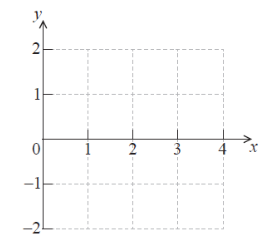
\includegraphics[scale=0.5]{repere_x23a}\par
    \noindent Repère pour la question a)\par
  \end{center} % or flushleft or flushright
  \begin{enumerate}[label=(\alph*)]
    \item Esquissez la représentation graphique de $g$ sur le repère.\hspace*{\fill} [4]
    \item À partir de là, trouvez la valeur de x pour laquelle $g(x) = -1$.\hspace*{\fill} [2]
  \end{enumerate}
\end{question}
